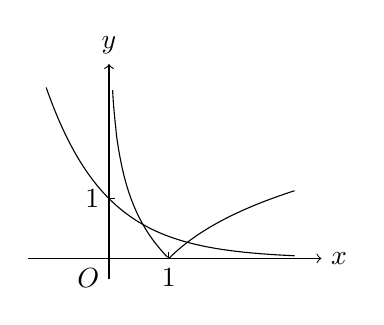
\begin{tikzpicture}[x=.76cm,y=.76cm,baseline=(current bounding box.center)]
  \draw[->] (-1.35,0)--(3.55,0) node[right] {$x$}; \draw[->] (0,-.35)--(0,3.25) node[above] {$y$};
  \draw[domain=-1.05:3.1,samples=100,smooth] plot (\x,{exp(-\x)});
  \draw[domain=.06:.98,samples=100,smooth] plot (\x,{-ln(\x)});
  \draw[domain=1:3.1,samples=100,smooth] plot (\x,{ln(\x)});
  \draw (1,0)--(1,.10) (0,1)--(.10,1);
  \node[below] at (1,0) {$1$}; \node[left] at (0,1) {$1$}; \node[below left] at (0,0) {$O$};
\end{tikzpicture}
